\chapter{Выделение области радужки на изображении}
\label{chapter:segmentation}

Выделение (сегментация) области радужки на изображении -- один из основных этапов распознавания. Ошибки сегментации влекут за собой рост числа ошибок распознавания, делая систему менее надежной и удобной в использовании. Подавляющее большинство существующих подходов ориентированы на использование систем в условиях слабо изменяющегося окружения. Классические методы, основанные на эвристиках, хорошо зарекомендовали себя здесь. Широкое распространение технологий распознавания создает необходимость обеспечения полной функциональности систем в более широком диапазоне условий и, как следствие, создания более гибких и устойчивых решений.

\section{Особенности выделения радужки в сложных условиях}
\label{sec:hard_condition_segm_features}

Сложные условия окружения, характерные для сценария взаимодействия пользователя с мобильным устройством, оказывают значительное влияние не только на свойства самого биометрического признака, но и на качественные характеристики изображения, из которого следует предварительно извлечь информацию, описывающую его уникальные особенности.

Факторы окружения в особенной степени существенны для биометрической системы, использующей изображение объекта распознавания в качестве входных данных, в особенной при распознавании по радужке: уровень окружающего освещения варьируется в диапазоне от $10^{-4}$ в ночное время суток или темном помещении до $10^5$ (лк) в полдень под прямыми солнечными лучами; распределение освещенности в области радужки, определяемое характеристиками и расположением источников света относительно лица и радужки. Изменение размеров зрачка приводят к деформации структуры радужки, различные погодные условия вынуждают пользователя устройства моргать, сильно прищуривать глаза и могут значительно снизить качество изображения в целом. Факторы окружения, влияющие на распознавание, подробно описаны в литературе~\cite{raja_2014,thavalengal_2016,btas_competition_2016,odinokikh_2018}, а некоторые примеры изображений радужки, получаемых в сложных условиях, приведены на Рис.~\ref{fig:iris-mobile-img-examples} и~\ref{fig:iris_iamge_quality_degradation}.

\begin{figure}[t!]
	\centering
	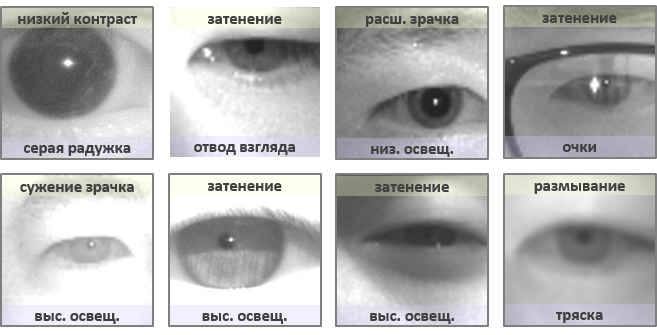
\includegraphics[width=0.95\columnwidth]{pictures/iris-mobile-img-examples.png}
	\caption{Примеры изображений полученных при помощи мобильного устройства: причина (снизу) и следствие (сверху)}
	\label{fig:iris-mobile-img-examples}
\end{figure}

Важной особенностью распознавания при помощи мобильного устройства являются поведенческие характеристики пользователя, описанные в главах~\ref{sec:mobile_iris_features} и~\ref{sec:main_difficulties_mobile}. Примеры ошибок выделения области радужки на изображении в следствие влияния факторов окружения и особенностей поведения пользователя приведены на Рис.~\ref{fig:iris_iamge_quality_degradation}.

\section{Методы выделения радужки на изображении}
\label{sec:segm_method}

\subsection{Обзор существующих методов}
\label{sec:segm_existing_app_overview}

Существует большое количество различных методов и подходов к решению задачи выделения области радужной оболочки глаза на изображении. Методы хорошо зарекомендовали себя для не мобильных приложений. Многие из них используются в коммерческих решениях и распространены настолько широко, что их по праву можно называть классическими.

Среди классических методов можно выделить основные направления:
\begin{enumerate}
	\item[$\bullet$] Применение интегро-дифференциального оператора (\ref{eq:daugman_ido}), предложенного в работе~\cite{daugman_how_works}. Оператор используется для выделения радиально-симметричных структур, которыми, в данном случае, предлагается описывать зрачок и радужку. Метод имеет высокие точность и устойчивость, но обладает неприемлемой для большинства приложений вычислительной сложностью~\cite{matveev_doctor_thesis}. Примеры использования~\cite{bakhtiari_2006,adam_2008,barzegar_2008}. Примеры совершенствования исходного решения путем добавления различных методов предобработки представлены в работах~\cite{alonso_11,alonso_12,hu_11,jeong_10,mahadeo_12};
	\item[$\bullet$] Анализ гистограммы изображения, бинаризации и последующее оценивание радиусов зрачка и радужки~\cite{guang_2007,pan_2007,ling_2010}. Методы показали свою работоспособность на качественных изображениях~\cite{casia_v3,bath_2005}, однако, в сложных условиях~\cite{ndiris_2010,ubiris_2005} их применение сильно ограничено;
	\item[$\bullet$] Методология Хафа (Hough), позволяющая оценить параметры кривых заданного вида (в данном случае окружностей, описывающих зрачок и радужку) с использованием т.н. аккумуляторов. В качестве примеров использования различных подходов внутри методологии можно привести следующие~\cite{wildes_1997,proenca_2006,basit_2007,boyd_2010}. Данный подход позволяет получить выигрыш по скорости обработки, но гораздо менее устойчив к зашумлённым данным в сравнении, например, с методами, использующими интегро-дифференциальный оператор.
\end{enumerate}

Существенная часть работ, посвящённых выделению области радужки за последнее время и приходящаяся на период с 1997 по 2014 годы, сосредоточена вокруг вышеперечисленных методов~\cite{korobkin_odinokikh_segm_2018}. В работах предлагаются различные варианты улучшения методологий путем добавления процедуры специальной предобработки изображения~\cite{yuan_2005,pan_2007}, решающих правил, основанных на всевозможных эвристиках~\cite{matveev_doctor_thesis,daugman_how_works,ma_2004,zhou_2004,bowyer_survey_2008,moravcik_2010}, а также техник машинного обучения. Общая схема классического подхода изображена на Рис.~\ref{fig:segm-classic-approach} Методы хорошо разобраны и классифицированы по различным особенностям в работе~\cite{matveev_doctor_thesis}.

\begin{figure}[h!]
	\centering
	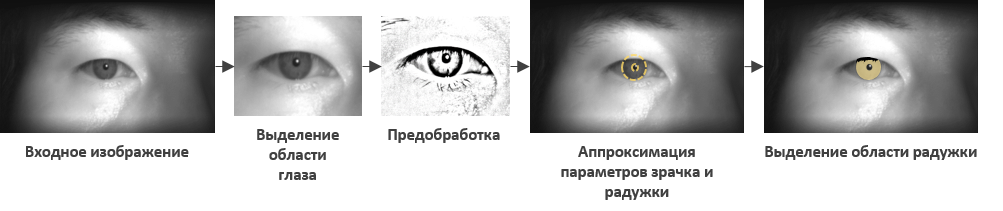
\includegraphics[width=0.95\columnwidth]{pictures/segm-classic-approach.png}
	\caption{Общая схема классического подхода к выделению радужки на изображении)}
	\label{fig:segm-classic-approach}
\end{figure}

С увеличением количества всевозможных данных для обучения и развитием аппаратных средств область машинного обучения в недавнем времени претерпела существенные изменения. Глубокое обучение (deep learning, DL) стало одним из подходов, позволяющих эффективно использовать данные большие объемы данных. Начиная с 2012 года глубокое обучение и, в частности, глубокие сверточные нейронные сети (deep convolutional neural networks, deep CNN) были успешно применены для решения целого ряда задач компьютерного зрения, достигнув результатов, в значительной степени превосходящих полученный ранее существующими методами и даже человека~\cite{krizhevsky_2012,girshick_2014,toshev_2014,karpathy_2014}.

Прошло некоторое время, пока глубокое обучение достигло области биометрического распознавания и было применено для выделения радужки на изображении. На сегодняшний день создание различных приложений, в том числе мобильных, требует от алгоритма высокой устойчивости к сильно изменяющимся условиям окружения, упомянутым ранее (\ref{sec:main_difficulties_mobile}). Авторы~\cite{liu_2016} впервые продемонстрировали преимущества подхода к сегментации радужки с использованием свёрточных нейронных сетей, в частности, на изображениях радужек, полученных в более сложных условиях. В работе также сравниваются два основных подхода к сегментации с использованием сверточных сетей: так называемый <<patch-based>> подход, при котором сеть обучают с использованием небольших фрагментов исходного изображения, принадлежащих либо не принадлежащих области объекта, который необходимо выделить, присваивая каждому из фрагментов марку класса в зависимости от принадлежности; вторым подходом является т.н. <<end-to-end>> способ обучения, когда на вход сети подается полноразмерное изображение, а выходом её является бинарная маска той же размерности, значение каждого пикселя в которой определяет класс объекта, например: 1 - радужка, 0 - фон.

Иным примером <<patch-based>> подхода является архитектура, представленная в работе~\cite{arsalan_2017}. Незадолго до её появления, исследователи в~\cite{shelhamer_2017} показали, что такой подход и предложенный метод обучения в значительной степени ухудшают качество сегментации, в очередной раз закрепив преимущества <<end-to-end>> подхода. В работе~\cite{jalilian_2017} продемонстрирована возможность использования архитектуры SegNet применительно к сегментации радужки, а также предложено использование техники дропаут (dropout) обучения, впервые описанной в работе~\cite{wang_2013}. Подход позволил достигнуть достаточно высокой точности сегментации, однако, в виду вычислительной сложности, не применим на практике. Иная CNN архитектура была представлена в работе~\cite{bazrafkan_2018}. Предложено исключение пулинг (pooling) слоёв, показана высокая эффективность. Однако, в работе~\cite{krizhevsky_2012} ранее утверждалось, что такой подход не позволяет извлекать сложные особенности из изображения, что критично для задачи сегментации в сложных условиях. Известно также, что отсутствие пулинг слоёв приводит к тому, что построенная на таком подходе архитектура оказывается чувствительной к различным сдвигам объекта на изображении.

\subsection{Выделение области радужки методами глубокого обучения}
\label{sec:segm_proposed_method}

В настоящей работе предложены новые CNN архитектуры. За основу взяты две базовые архитектуры, демонстрирующие лучшие результаты в задаче сегментации различных объектов на изображении: FCN (fully-convolutional network) и SegNet. Предложена новая структура основных блоков, из которых состоят обе архитектуры.

{\bf Основные подходы с использованием глубокого обучения}
\label{sec:segm_basic}

Архитктура FCN, впервые предложенная для решения задач семантической сегментации объектов, подразумевает полное исключение полносвязных (fully-connected) слоев~\cite{shelhamer_2017}. Это свойство позволяет адаптировать модель, обученную для решения задачи классификации, в модель, решающую задачу сегментации объектов без дополнительных оптимизаций. Архитектура поддерживает оба (patch-based и end-to-end) подхода к обучению и представляет собой модель т.н. <<кодировщик-декодировщик>> (encoder-decoder), изображенную на Рис.~\ref{fig:encoder-decoder-architecture}. Роль кодировщика заключается в построении высокоуровневого представления входных данных, в то время как декодировщик осуществляют обратную задачу. Принимая на вход представление, полученное кодировщиком, декодировщик переводит его в пространство размерности исходного изображения, используя закодированную информацию о пространственном соотношении различных элементов текстуры изображения.
В архитектуре FCN декодировщик построен с использованием блоков, содержащих слои деконволюции или (deconvolution layers) или транспонированные свёрточные слои, предложенные в работе~\cite{zeiler_2011}.
Выход каждого деконвоюционного слоя объединяется с картами признаков соответствующих симметричных слоёв кодировщика с использованием т.н. пропускных соединений (skip-connections) (Рис.~\ref{fig:encoder-decoder-architecture}) с целью восстановления структурной информации.

\begin{figure}[t!]
	\centering
	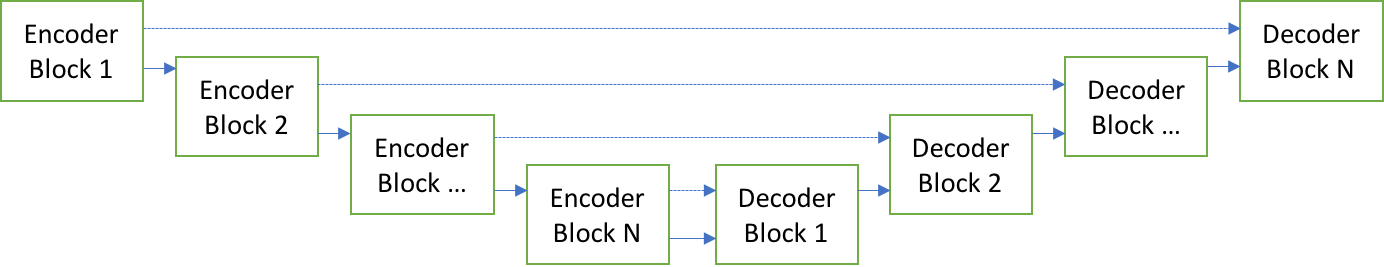
\includegraphics[width=0.95\columnwidth]{pictures/dec_enc.png}
	\caption{Общая схема архитектуры кодировщик-декодировщик (encoder-decoder)}
	\label{fig:encoder-decoder-architecture}
\end{figure}

Другим примером архитектуры, реализующей схему кодировщик-декодировщик выступает SegNet~\cite{badrinarayanan_2017}. Основным вкладом работы стала замена вычислительно-сложных и требовательных к памяти устройства операций деконволюции так называемыми <<unpooling>> слоями. Большая требовательность по объему потребляемой памяти для FCN обусловлена тем необходимостью хранить карты признаков, являющихся выходами каждого из блоков кодировщика до тех пор, пока они не будут использованы декодировщиком. Таким образом, пик потребления памяти устройства архитектурой достигается в момент, когда все карты признаков кодировщика извлечены, т.е. в момент формирования вышеупомянутого высокоуровневого представления. Архитектура SegNet позволяет на порядки снизить количество памяти, необходимой для полного прямого прохода. Несмотря на преимущества, подход SegNet с unpooling слоями снижает емкость сети, а невозможность пропускать градиенты через skip-connection при обратном распространении ошибки затрудняют обучение. Разница между структурами блоков декодировщика FCN и SegNet проиллюстрирована на Рис.~\ref{fig:fcn-segnet}.

\begin{figure}[t!]
	\centering
	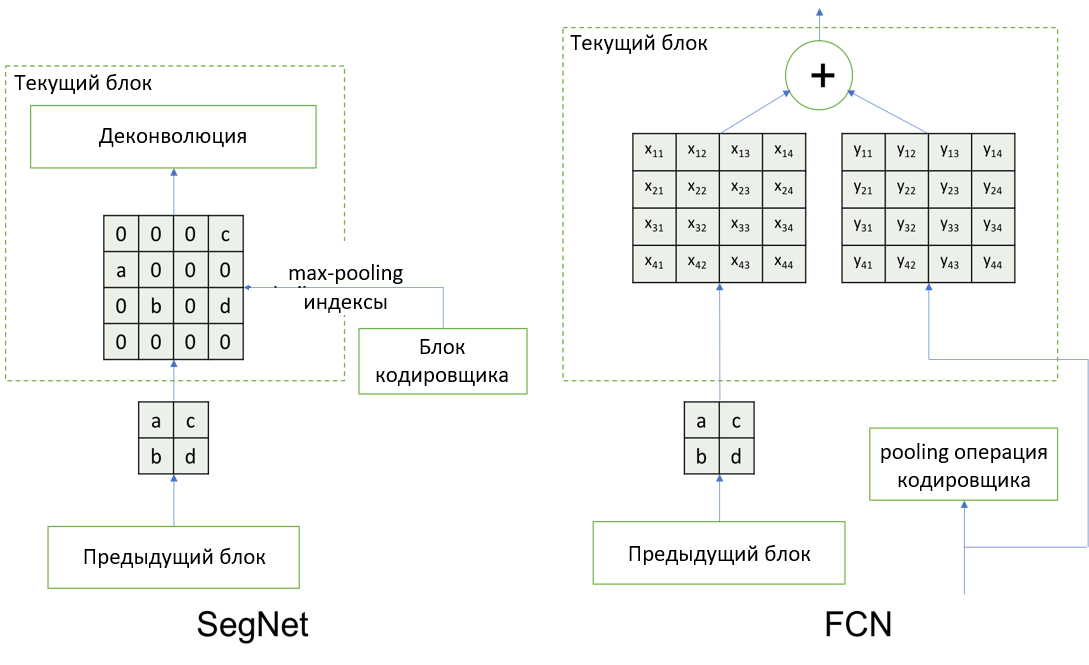
\includegraphics[width=0.95\columnwidth]{pictures/fcn_segnet.png}
	\caption{Структуры основных блоков декодировщиков FCN (справа) и SegNet (слева)}
	\label{fig:fcn-segnet}
\end{figure}

{\bf Структура основных блоков архитектуры}
\label{sec:segm_proposed_blocks}

Изначально идея использования остаточных (residual) связей при конструировании блоков была предложена в контексте очень глубоких сетей~\cite{he_2016}. Далее, остаточные блоки хорошо зарекомендовали себя как эффективно использующие память и позволяющие при этом поддерживать достаточную ёмкость. Их обходные (bypass) соединения способствуют эффективной передаче градиента при обратном распространении и позволяют оптимизировать также добавочную часть в каждом соединении. Общая структура остаточного блока приведена на Рис.~\ref{fig:gen-resnet}. Авторы~\cite{he_2016} также предложили сразу несколько модификации блока, отличающихся количеством каналов и глубиной (Рис.~\ref{fig:res-types}).

\begin{figure}[h!]
	\centering
	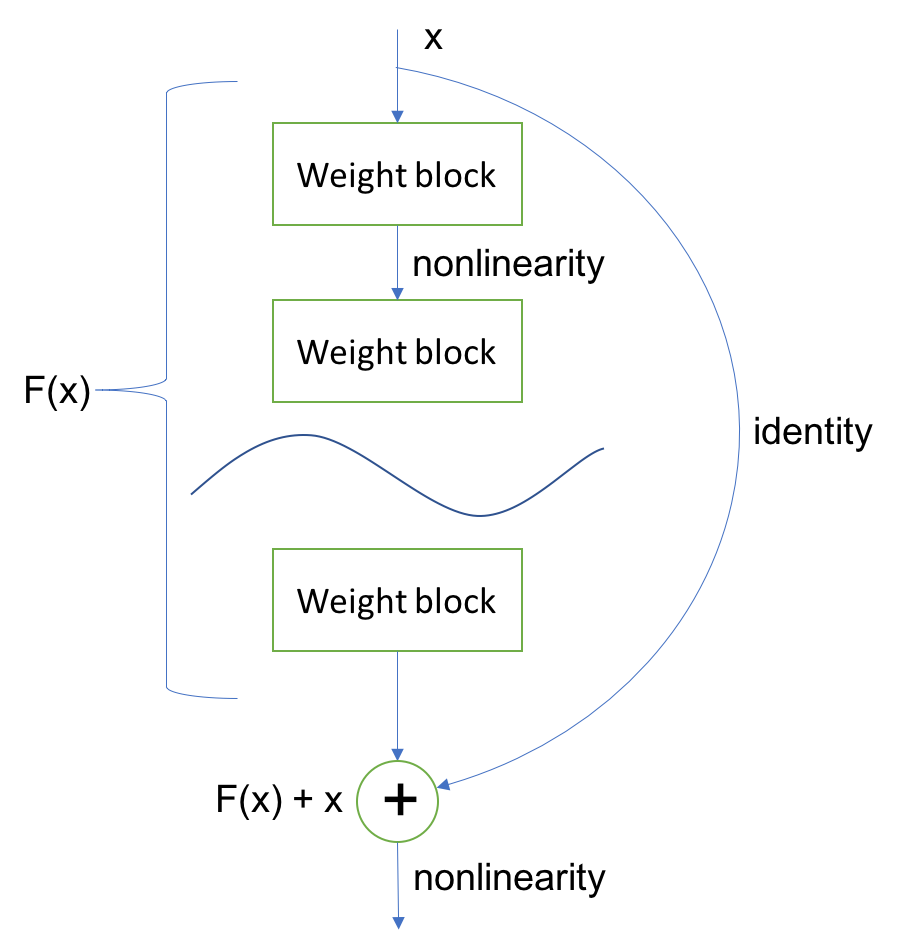
\includegraphics[width=0.45\columnwidth]{pictures/general_resnet.png}
	\caption{Общая структура остаточного (residual) блока}
	\label{fig:gen-resnet}
\end{figure}

Предложено дополнение блоков слоями нормализации (batch normalization), впервые описанными в работе~\cite{ioffe_2015}, позволяющими ускорить сходимость модели и повысить её обобщающую способность, тем самым снижать чувствительность модели к вариациям входных данных.

\begin{figure}[t!]
	\centering
	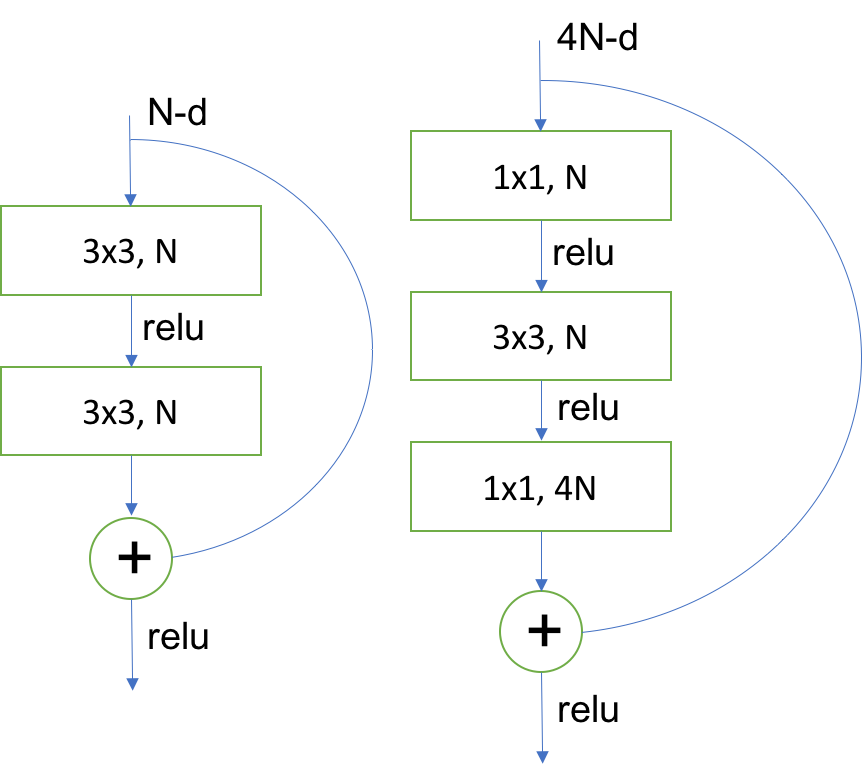
\includegraphics[width=0.5\columnwidth]{pictures/res_types.png}
	\caption{Модификации остаточных (residual) блоков: simple - слева, bottleneck - справа}
	\label{fig:res-types}
\end{figure}

{\bf Предложенные архитектуры}
\label{sec:segm_proposed_architecture}

Обе вышеупомянутые архитектуры (FCN, SegNet) были взяты за основу и модифицированы. SegNet по заявлению авторов~\cite{badrinarayanan_2017} позволяет обеспечить относительно низкое потребление памяти, хотя это во многом зависит от целевой платформы и вычислительных средств. С другой стороны FCN демонстрирует лучшую показатели сходимости. Архитектура ResNet-26 с блоками типа simple была взята в качестве кодировщика и симметрично-отражённая (Рис.~\ref{fig:encoder-decoder-architecture}) как декодировщик для модифицированной FCN. Предложенная модификация SegNet представляет собой ResNet-18 кодировщик и симметрично-отражённый декодировщик (Рис.~\ref{fig:encoder-decoder-architecture}). Блоки типа bottleneck были исключены из рассмотрения для применения в FCN, т.к. требовательны к размеру карт признаков на каждом последнем слое, что является существенной проблемой для FCN. Для FCN все слои max-pooling были заменены большими значениями смещений ядра в сверточных слоях (strided convolutions). В случае с SegNet max-pooling слои были перемещены в конец каждого блока кодировщика, а смещения ядер были выбраны единичными.

{\bf Экспериментальные результаты}
\label{sec:segm_exp_results}

Экспериментальные результаты были получены на двух наборах данных: публично доступном CASIA-Iris-Lamp-V3~\cite{casia_v3_lamp} и его модификации. Для оценки качества сегментации был выбран коэффициент Жаккара (Jacсard Index, IoU - intersection over Union,~\ref{eq:jaccard_index})~\cite{shelhamer_2017}. В качестве метода для сравнения был выбран метод, демонстрирующий наилучшие результаты~\cite{liu_2016}.

\begin{equation}
\label{eq:jaccard_index}
J(I_{pr},I_{gt}) = \frac{|I_{pr} \cap I_{gt}|}{|I_{pr} \cup I_{gt}| } = \frac{|I_{pr} \cap I_{gt}|}{|I_{pr}|+|I_{gt}|-|I_{pr} \cap I_{gt}|},
\end{equation}

\noindent
где $I_{pr}$ и $I_{gt}$  - множества пикселей, принадлежащих области радужки, предсказанных моделью и размеченными экспертом соответственно.

База данных изображений радужек CASIA-Iris-Lamp-V3 была выбрана в качестве основной для тестирования. Особенность этой БД в том, что в ней представлены изображения, полученные в осложненных, изменяющихся условиях окружения, позволяющие симулировать внутриклассовые отклонения: различные размеры зрачков, отвод взгляда, перепады яркости и др. База данных содержит 16212 изображений радужек 411 субъектов. Для оценивания методов были случайным образом выбраны 4865 изображений 124 субъектов. Разметка произведена экспертом с выполнением следующих условий: все пиксели, принадлежащие области радужки на изображении, а также ресницы, пересекающие область радужки, были приняты относящимися к классу <<область радужки>> (Рис.~\ref{fig:seg-results}). Область ресниц, перекрывающих радужку на изображении была также отнесена к классу радужки т.к. одной из основных целей работы было показать преимущества предложенных архитектур по сравнению с существующими. Сценарий был выбран именно таким, потому что позволил существенно упростить процедуру разметки и, таким образом, увеличить количество данных. База данных была предварительно поделена на три подвыборки: обучающую (train), валидационную (validation) и тестовую (test) в соотношении 3386, 478 и 1001 изображений соответственно. Результаты, полученные на валидационной выборке, использовались для выбора лучшей модели, которая затем оценивалась на тестовой.

\begin{figure}[t!]
	\centering
	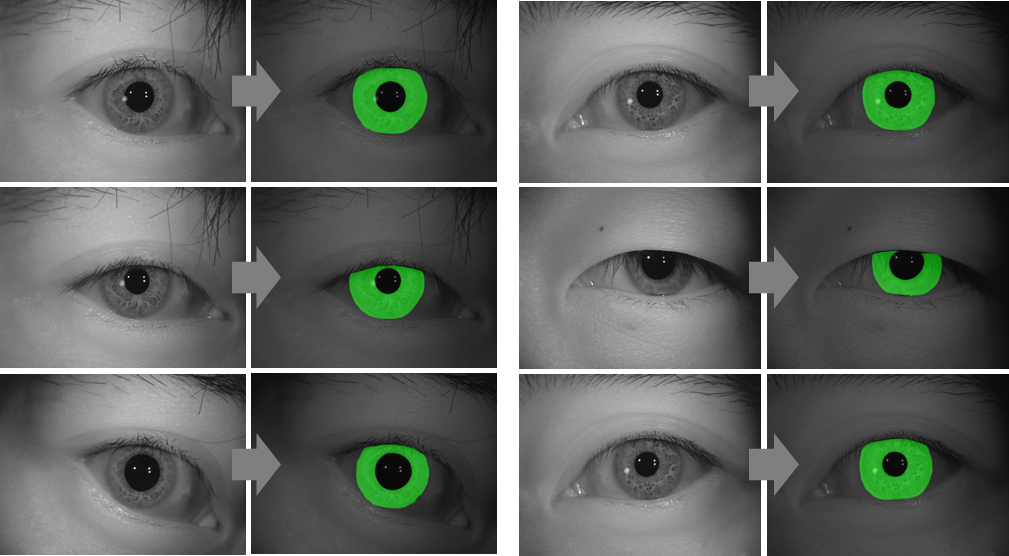
\includegraphics[width=0.95\columnwidth]{pictures/seg-results.png}
	\caption{Результаты выделения области радужки}
	\label{fig:seg-results}
\end{figure}

Исследуемые модели обучались на протяжении 200 эпох пакетами (batch) изображений по 8 штук. В качестве алгоритма оптимизации был выбран Adam~\cite{kingma_2014}. Параметры обучения и тестирования были выбраны одинаковыми для всех исследуемых моделей.

Было проведено два эксперимента. В первом модели обучались на БД~\cite{casia_v3_lamp} без модификаций. Результаты представленные в Таб.~\ref{tab:seg-results}, демонстрируют что обе предложенные модели показывают примерно одинаково хорошие результаты, незначительно превосходя модель~\cite{liu_2016}.

\begin{equation}
\label{eq:random_contrast}
I'(x,y) = (I(x,y) - \overline{I}) \cdot C + \overline{I},
\end{equation}

\noindent
где $I(x,y)$ - исходное изображение, $\overline{I}$ - среднее значение яркости исходного изображения, $C$ - коэффициент изменения контраста.

Целью второго эксперимента была симуляция еще более значительных изменения окружения. С этой целью над исходным набором обучающих данных была произведена операция аугментации. Для этого над каждым изображением в обучающей выборке были выполнены следующие операции: значение контраста $C$ изменялось случайным образом в диапазоне $[50\%, 150\%]$ (~\ref{eq:random_contrast}), случайное значение в диапазоне $[-20\%, 20\%]$ также присваивалось интенсивности каждого пикселя. Финальное тестирование производилось на оригинальных изображениях из БД. Результаты показали, что предложенные модели значительное превосходят MFCN~\cite{liu_2016}, демонстрируя высокую устойчивость к изменениями условий окружения, а также высокую обобщающую способность. Несколько примеров результатов сегментации радужки на изображениях из CASIA-Iris-Lamp-V3 представлены на Рис.~\ref{fig:seg-results}.

\begin{table}[t]
	\begin{center}
		\begin{tabular}{|l|c|c|c|c|}
			\hline
			\multirow{2}{*}{Модель} & \multicolumn{2}{|c|}{Исх. набор данных, IoU} & \multicolumn{2}{|c|}{Модиф. набор данных, IoU} \\ \cline{2-5}
			\space 	& val. 	& test 	& val. 	& test set \\ \hline
			MFCN 	& $0.918$ 				& $0.919$ 				& $0.668$ 				& $0.676$ \\ \hline
			FCN 	& $0.930$ 				& $0.930$ 				& $0.884$ 				& $0.894$ \\ \hline
			SegNet 	& $0.928$ 				& $0.929$ 				& $0.916$ 				& $0.924$ \\ \hline
		\end{tabular}
		\caption{Результаты по точности выделения области радужки на изображении}
		\label{tab:seg-results}
	\end{center}
\end{table}

{\bf Результаты по скорости распознавания}
\label{sec:segm_results_speed}

Производительность метода оценивалась на процессоре Qualcomm Snapdragon 835 (2.45 GHz). Медианное время выполнения составило 35 мсек. Алгоритмическая сложность метода, при условии фиксирования её параметров (весов и смещений) и добавления операции масштабирования на входе, линейна по размеру входных данных.

\section{Выводы ко второй главе}

Рассмотрены особенности выделения области радужной оболочки глаза на изображениях, получаемых в сложных условиях окружения, связанных с использованием мобильного устройства и взаимодействия с пользователем. Приведен обзор и классификация существующих методов, обозначены их основные преимущества и недостатки. Рассмотрены новые методы, построенные с использованием методов глубокого обучения, выделены их основные преимущества, подчеркнуты перспективы использования и развития. Предложены, протестированы две новые архитектуры сверточных нейронных сетей, позволяющих производить устойчивое выделение области радужки на изображении низкого качества в сложных условиях окружения с частотой поступления кадров (15 кадров в секунду). Обе архитектуры позволили превзойти существующие, известные из литературы решения, основанные на глубоком обучении. Одна из предложенных архитектур успешно внедрена и используется в коммерческих продуктах.